
\begin{figure}
\caption{\label{fig:median_period} Period lengths}
	\centering
	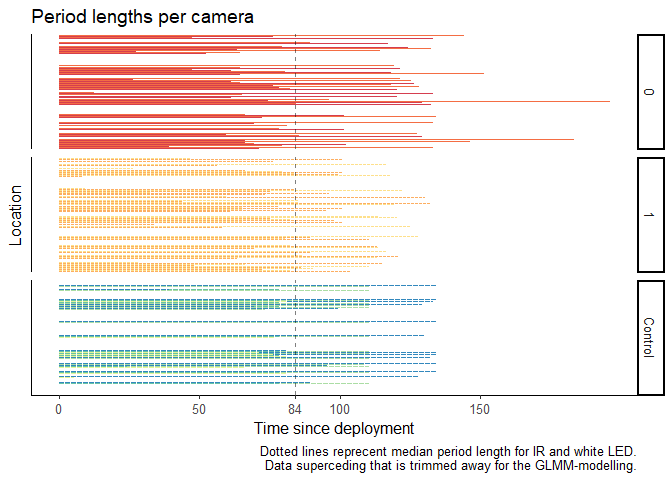
\includegraphics[scale=.8]{../R/glmm_sp_files/figure-gfm/period-length-wControl-1.png}
\end{figure}


\begin{figure}
	\begin{subfigure}{1\textwidth}
		\centering
		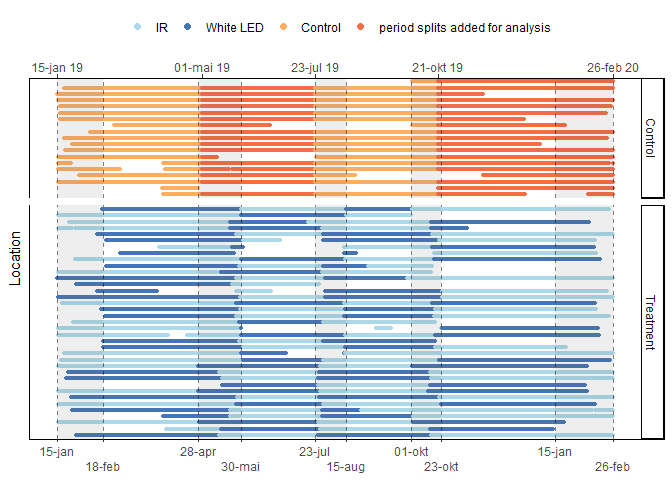
\includegraphics[scale=.8]{../R/FLM_notebook_files/figure-gfm/effort-facet-1.png}
			\caption{\label{fig:timeseries_flash} Cameras with white LED periods}	
	\end{subfigure}	
	\begin{subfigure}{1\textwidth}
		\centering
		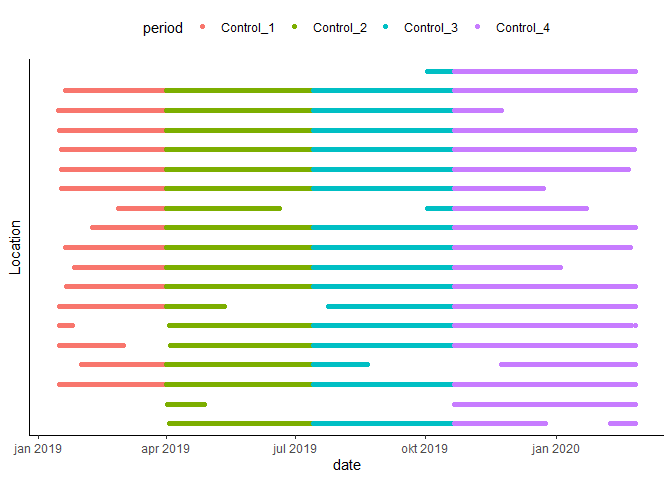
\includegraphics[scale=.8]{../R/FLM_notebook_files/figure-gfm/effort-facet-2.png}
			\caption{\label{fig:timeseries_control} Control cameras'\\ period breaks were set during the analysis.}	
	\end{subfigure}	
\caption[Active camera days]
{Colours indicate the different periods for each camera. Control camera periods were defined in similar lengths to that of the cameras that had periods with an additional white LED CT. Thus, "day 0" of Control-cameras are often set at dates far from an actual visitation day. \label{fig:timeseries_figure}}
\end{figure}
